\documentclass[border=8pt]{standalone}
\usepackage{amsmath,amssymb}
\usepackage{tikz}
\usetikzlibrary{arrows.meta,calc,decorations.pathreplacing,patterns,shapes.geometric,positioning,shadings}

\begin{document}
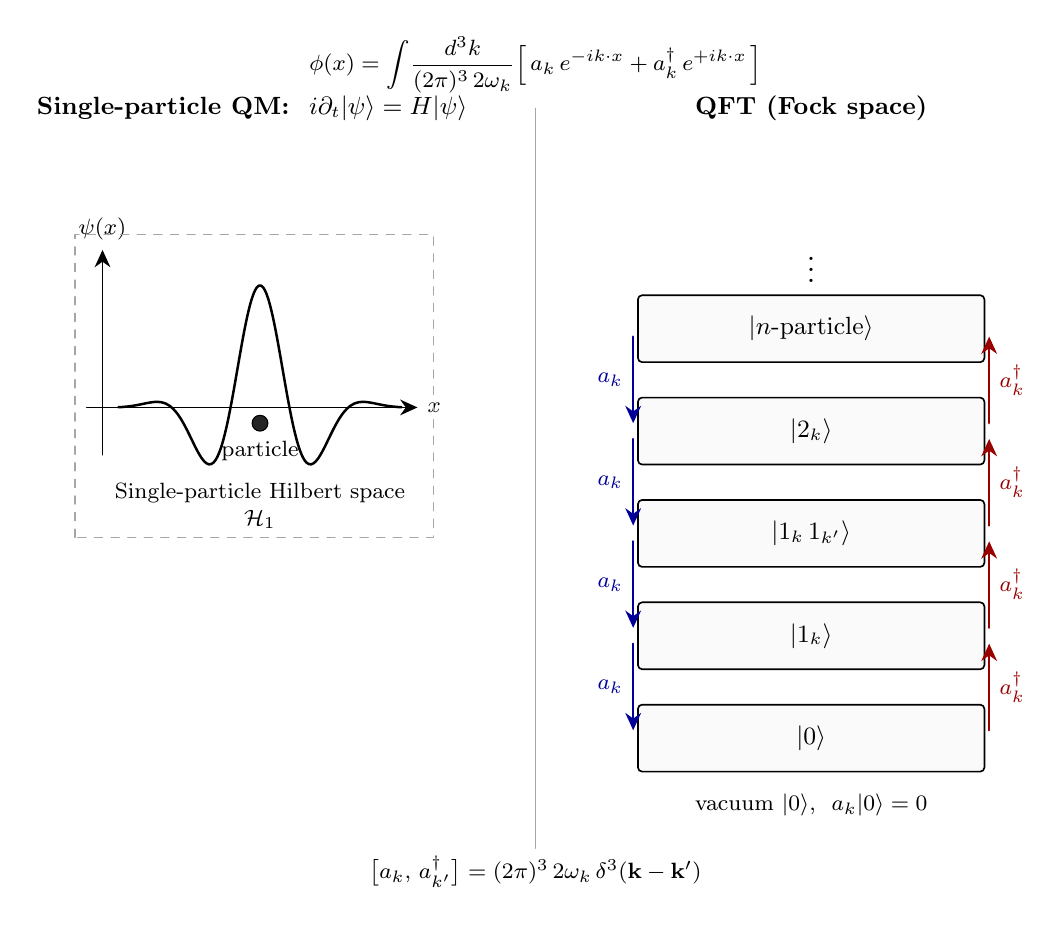
\begin{tikzpicture}[
    >={Stealth[length=2.2mm,width=2mm]},
    line cap=round,line join=round,
    every node/.style={font=\small},
    creop/.style={->,thick,color=red!60!black},
    annop/.style={->,thick,color=blue!60!black},
    layer/.style={draw=black,line width=0.6pt,rounded corners=1.5pt,
                  minimum width=4.4cm,minimum height=0.85cm,fill=black!2},
    sectitle/.style={font=\small\bfseries},
]

% ===== Top formula band =====
\node[align=center,font=\footnotesize] at (3.0,7.55)
  {$\displaystyle \phi(x)=\int\!\frac{d^{3}k}{(2\pi)^{3}\,2\omega_k}\Big[\,a_k\,e^{-ik\cdot x}+a_k^{\dagger}\,e^{+ik\cdot x}\,\Big]$};

% ===== Vertical separator =====
\draw[gray!70,line width=0.4pt] (3.0,-2.4) -- (3.0,7.0);

% ===== Section titles =====
\node[sectitle] at (-0.6,7.0) {Single-particle QM:\ \ $i\partial_t|\psi\rangle=H|\psi\rangle$};
\node[sectitle] at (6.5,7.0)  {QFT (Fock space)};

% ============================================================
% LEFT COLUMN: Single-particle Hilbert space
% ============================================================

% wavefunction axes
\draw[->,line width=0.6pt] (-2.7,3.2) -- (1.5,3.2) node[right,font=\footnotesize]{$x$};
\draw[->,line width=0.6pt] (-2.5,2.6) -- (-2.5,5.2) node[above,font=\footnotesize]{$\psi(x)$};

% wavefunction curve (gaussian-like wavepacket with oscillation)
\draw[line width=0.9pt,smooth,domain=-2.3:1.3,samples=120,variable=\x]
  plot ({\x},{3.2 + 1.55*exp(-1.6*(\x+0.5)*(\x+0.5))*cos(deg(4.2*(\x+0.5)))});

% small particle icon
\filldraw[fill=black!85,draw=black] (-0.5,3.0) circle (0.10);
\node[font=\footnotesize] at (-0.5,2.65) {particle};

\node[font=\footnotesize,align=center] at (-0.5,1.95)
  {Single-particle Hilbert space\\ $\mathcal{H}_{1}$};

% box around wavefunction region
\draw[dashed,gray!70] (-2.85,1.55) rectangle (1.7,5.4);

% ============================================================
% RIGHT COLUMN: Fock space tower
% ============================================================

% Layers (bottom -> top)
\node[layer] (l0) at (6.5,-1.0) {$|0\rangle$};
\node[layer] (l1) at (6.5, 0.3) {$|1_{k}\rangle$};
\node[layer] (l2) at (6.5, 1.6) {$|1_{k}\,1_{k'}\rangle$};
\node[layer] (l3) at (6.5, 2.9) {$|2_{k}\rangle$};
\node[layer] (l4) at (6.5, 4.2) {$|n\text{-particle}\rangle$};

% ellipsis at top (infinite tower)
\node[font=\large] at (6.5,5.05) {$\vdots$};

% creation arrows (a^\dagger) on the right of the tower (going up)
\draw[creop] ($(l0.east)+(0.05,0.1)$) -- ($(l1.east)+(0.05,-0.1)$)
  node[midway,right,font=\footnotesize,color=red!60!black]{$a_{k}^{\dagger}$};
\draw[creop] ($(l1.east)+(0.05,0.1)$) -- ($(l2.east)+(0.05,-0.1)$)
  node[midway,right,font=\footnotesize,color=red!60!black]{$a_{k}^{\dagger}$};
\draw[creop] ($(l2.east)+(0.05,0.1)$) -- ($(l3.east)+(0.05,-0.1)$)
  node[midway,right,font=\footnotesize,color=red!60!black]{$a_{k}^{\dagger}$};
\draw[creop] ($(l3.east)+(0.05,0.1)$) -- ($(l4.east)+(0.05,-0.1)$)
  node[midway,right,font=\footnotesize,color=red!60!black]{$a_{k}^{\dagger}$};

% annihilation arrows (a) on the left of the tower (going down)
\draw[annop] ($(l1.west)+(-0.05,-0.1)$) -- ($(l0.west)+(-0.05,0.1)$)
  node[midway,left,font=\footnotesize,color=blue!60!black]{$a_{k}$};
\draw[annop] ($(l2.west)+(-0.05,-0.1)$) -- ($(l1.west)+(-0.05,0.1)$)
  node[midway,left,font=\footnotesize,color=blue!60!black]{$a_{k}$};
\draw[annop] ($(l3.west)+(-0.05,-0.1)$) -- ($(l2.west)+(-0.05,0.1)$)
  node[midway,left,font=\footnotesize,color=blue!60!black]{$a_{k}$};
\draw[annop] ($(l4.west)+(-0.05,-0.1)$) -- ($(l3.west)+(-0.05,0.1)$)
  node[midway,left,font=\footnotesize,color=blue!60!black]{$a_{k}$};

% vacuum annotation (below bottom layer)
\node[font=\footnotesize,align=center] at (6.5,-1.85)
  {vacuum $|0\rangle$,\ \ $a_{k}|0\rangle=0$};

% ===== Bottom commutator band =====
\node[align=center,font=\footnotesize] at (3.0,-2.7)
  {$\bigl[a_{k},\,a_{k'}^{\dagger}\bigr]=(2\pi)^{3}\,2\omega_{k}\,\delta^{3}(\mathbf{k}-\mathbf{k}')$};

\end{tikzpicture}
\end{document}
